\documentclass[12pt,twocolumn,letterpaper]{article}

\usepackage{cvpr}
\usepackage{times}
\usepackage{epsfig}
\usepackage{graphicx}
\usepackage{amsmath}
\usepackage{amssymb}
\usepackage[breaklinks=true,bookmarks=false]{hyperref}
\usepackage{subcaption}

\cvprfinalcopy

\def\httilde{\mbox{\tt\raisebox{-.5ex}{\symbol{126}}}}


\setcounter{page}{1}
\begin{document}

\title{3D Perspective Effects on a Smart Phone}

\author{Jai Prakash\\
Carnegie Mellon University\\
Master of Science in Computer Vision\\
{\tt\small jprakash@andrew.cmu.edu}
% For a paper whose authors are all at the same institution,
% omit the following lines up until the closing ``}''.
% Additional authors and addresses can be added with ``\and'',
% just like the second author.
% To save space, use either the email address or home page, not both
\and
Jennifer Lake\\
Carnegie Mellon University\\
Master of Science in Computer Vision\\
{\tt\small jelake@andrew.cmu.edu}
}

\maketitle
%\thispagestyle{empty}

%%%%%%%%% ABSTRACT
\begin{abstract}
In this project, we aim to create a 3D perspective transformation on a smart phone that will give the illusion of negative parallax.  The user should feel that there is depth to the smart phone screen, rather than just a flat screen (citation).   This is achieved by finding the three-dimensional vector between the user’s face and the center of the phone.  This was achieved by tracking the user’s face using the front-facing camera and calculating the smart phone’s orientation using the Internal Measurement Unit (IMU) and using Kalman filtering to smooth out the measurements.  Finally, these two pieces of information are combined to find the desired vector to create the perspective illusion.
\end{abstract}

\section{Introduction}
\subsection{Motivation}
As mobile phones have evolved over the last twenty years, many of the major milestones have been in display improvements. Mobile phones have gone from very small, simple displays to larger and more colorful displays.  At the forefront of this evolution, there is a growing trend of three-dimensional displays.  The primary motivation driving this trend in 3D perspective displays is to give the user more a more immersive user experience.

In 2013, Apple introduced the parallax effect on their line of iPhones, which allows for a 3D-like feeling, just short of a full 3D perspective effect \cite{BusinessInsider}.  In 2015, the Amazon Fire Phone introduced a full 3D perspective effect, which was branded as "Dynamic Perspective" \cite{DigitalTrends}.  It is this type of effect that we aim to create in this project however, unlike the Amazon Fire Phone, we will be implementing this effect on simpler, standard smart phone hardware
\subsection{Background}
    
\subsection{Related Work}
\subsubsection{Amazon Fire Phone}
     -Jenna
\subsubsection{Virtual Window}
     -Jenna
     
\begin{figure}
\begin{subfigure}{0.2\textwidth}
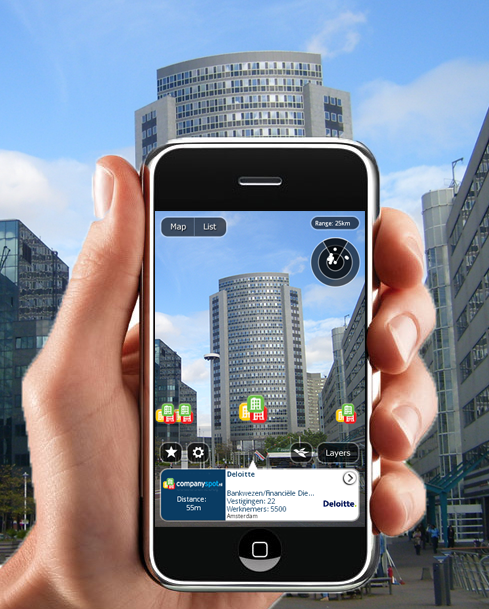
\includegraphics[scale=0.16]{images/AR_now}
\end{subfigure}
\begin{subfigure}{0.2\textwidth}
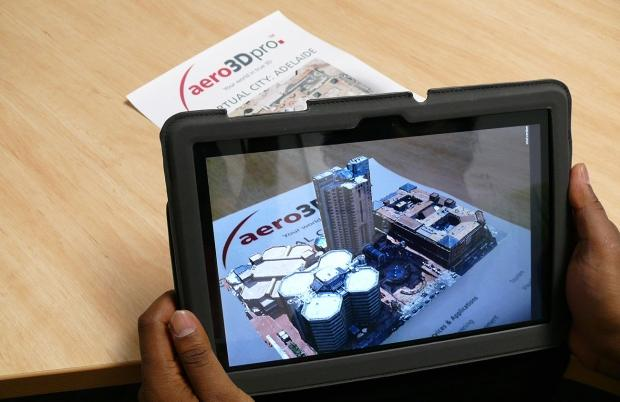
\includegraphics[scale=0.22]{images/AR_now1}
\end{subfigure}
\caption{AR in present smartphones}
\label{fig:arnow}
\end{figure}

\begin{figure}
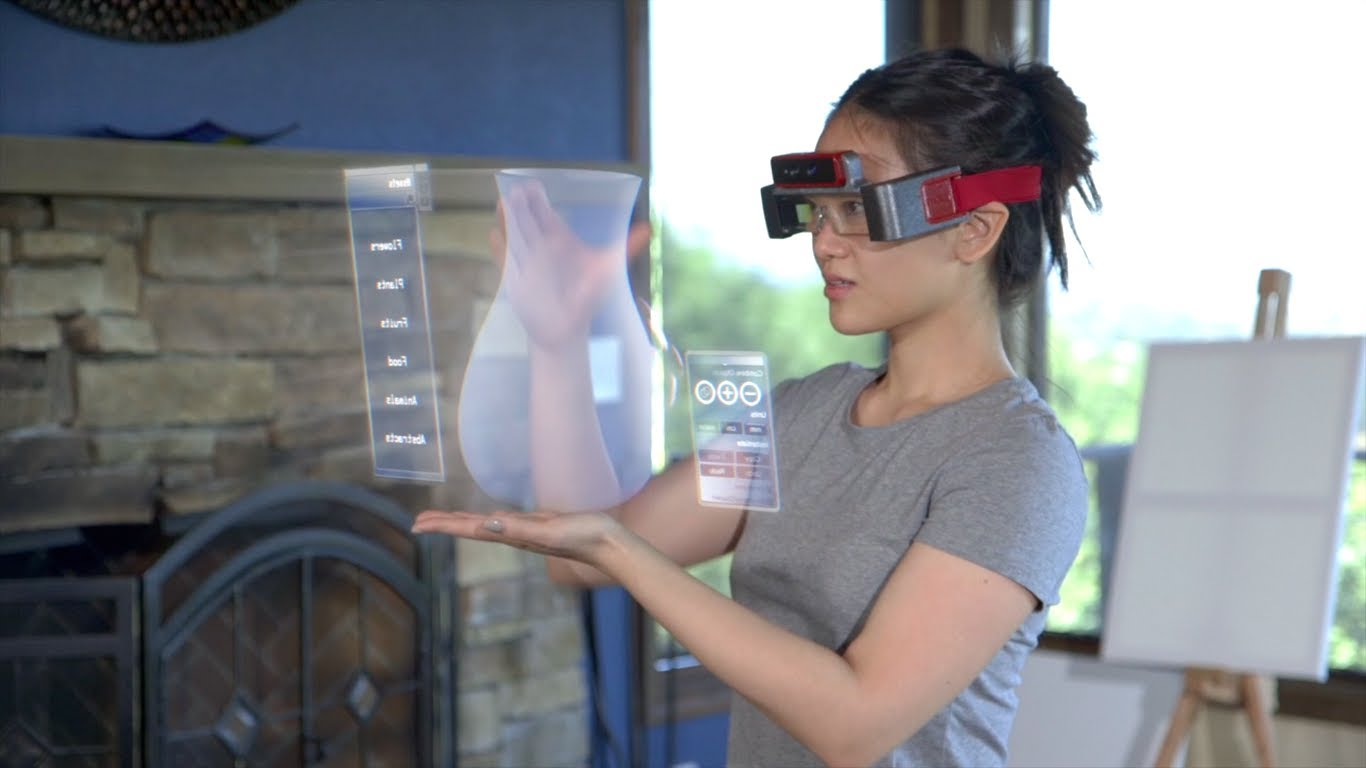
\includegraphics[scale=0.16]{images/mata}
\caption{Direct AR from Meta-glasses}
\label{fig:directar}
\end{figure}


\begin{figure}
\begin{subfigure}{0.22\textwidth}
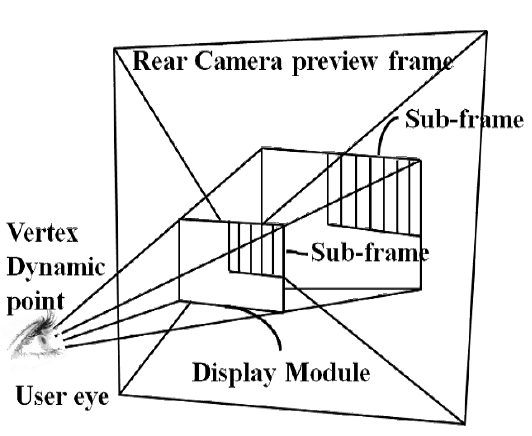
\includegraphics[scale=0.3]{images/transparenttablet}
\end{subfigure}
\begin{subfigure}{0.22\textwidth}
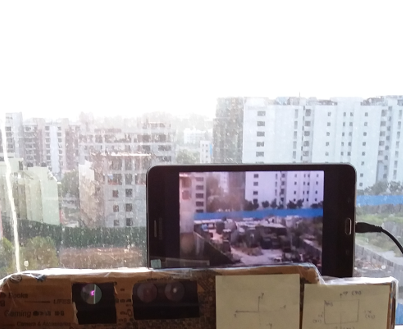
\includegraphics[scale=0.4]{images/transparenttablet1}
\end{subfigure}
\caption{Digital transparency using Kinect on Android tablet}
\label{fig:digitaltransparency}
\end{figure}

     
\subsubsection{Digital Transparency}
One more motivation for this project come from the augmented reality (AR) in present smartphones. The AR is smartphones can majorly be classified into two types
\begin{itemize}
\item \textbf{Indirect AR} Figure \ref{fig:arnow} shows augmented reality applications in current smartphones. This gives the user a video see-through experience, as the view is from the camera's perspective.
\item \textbf{Direct AR} These are the systems that give a perspective from user's point of view and hence give more immersive experience than indirect AR system. Holo-lens and meta-glasses (Figure \ref{fig:directar}) are examples of direct AR systems. 
\end{itemize}

The current direct AR systems are generally bulky and requires user to wear special glasses to use them. However, a direct AR system can be achieved in smartphones and tablets by using digital transparency \cite{jai}. Digital transparency system is shown in Figure \ref{fig:digitaltransparency}. This system tracks the eyes of the user and finds the angle which the tablet subtends at user's eye and crops the rear camera preview to the same angle to create a virtually transparent interface. This system gives a method to achieve direct AR on smartphones/tablets and hence gives a more immersive \textbf{glass-see-through} experience than conventional \textbf{video-see-through} experience.

This method uses a kinect sensor to track the accurate 3D position of the user with respect to tablet. The kinect sensor makes the system bulkier and difficult to use in smartphones. So, in this project we are addressing another method to achieve digital transparency using just the front facing camera and inertial sensors. A complete hands-free digital transparency system is out of scope of this project. The main concentration is on creating a dynamic perspective system which responds to the user's position with respect to the tablet.

\section{Method}
\begin{figure}
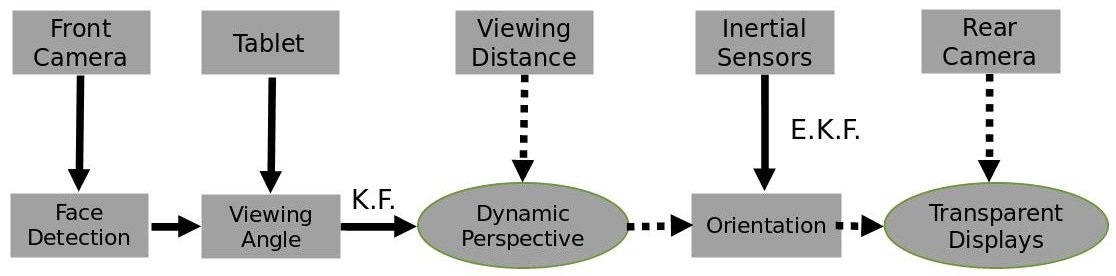
\includegraphics[scale=0.21]{images/block}
\caption{Block diagram of dynamic perspective system}
\label{fig:blockdia}
\end{figure}

Creating a dynamic perspective system involves finding the viewing angle of the user and rendering the graphical object depending on position of the user. This might involve three scenario
\begin{itemize}
\item Tablet is static and user moves
\item Tablet moves and user is static
\item Both tablet and the user can move
\end{itemize}

To find the motion and orientation of the phone, on-board inertial sensors can be deployed to find the orientation of the phone. A study on sensor fusion has been made to find the orientation of the phone.

The block diagram of the system is shown in the figure  \ref{fig:blockdia}. Solid arrow shows the algorithms implemented for this project. The dotted arrow parts are yet to be figured out to build a full fledge digital transparency system. However, the main focus is only on creating the dynamic perspective.

To create a dynamic perspective, we need to first track the position of user with respect to the tablet. In this project we assume that the distance of the eye from tablet is fixed (approximately 45-50 cm). This assumptions fails to address the scale factor in dynamic perspective. Hence, we don't get zoom-in and zoom-out effect as we move forward and backward. Since the distance from the tablet is assumed to be constant, we use the viewing angle to render the user interface (UI) in 3D. The following sections describe the exact methods used in each step.

\subsection{3D Geometry of Problem}
    -Jenna. describe the vectors involved
\subsection{Face Detection}
    -Jenna, I'm assuming this is Viola-Jones

\subsection{Kalman Filter}
The face detection using the cascade classifier is subject to jitter due to noise in the scene. The face detection sometimes fails because of various reasons like change is lighting conditions, change in expression of the face etc. This detection might cause jitter in the rendering. In order to avoid the jitter, we need to smooth the face detection and handle the no-detection case. The Kalman filter \cite{kalman}, can handle statistical uncertainties and other accuracies and produce results that are more accurate than a single measurement.

The Kalman filter models the uncertainties  in the states of position and velocities. The model alone is sufficient to predict the future uncertainties without remembering the past readings. which means that we can predict the state by knowing the parameters of the current state. Once the new reading arrive, the parameters of the model is updated.

\begin{figure}
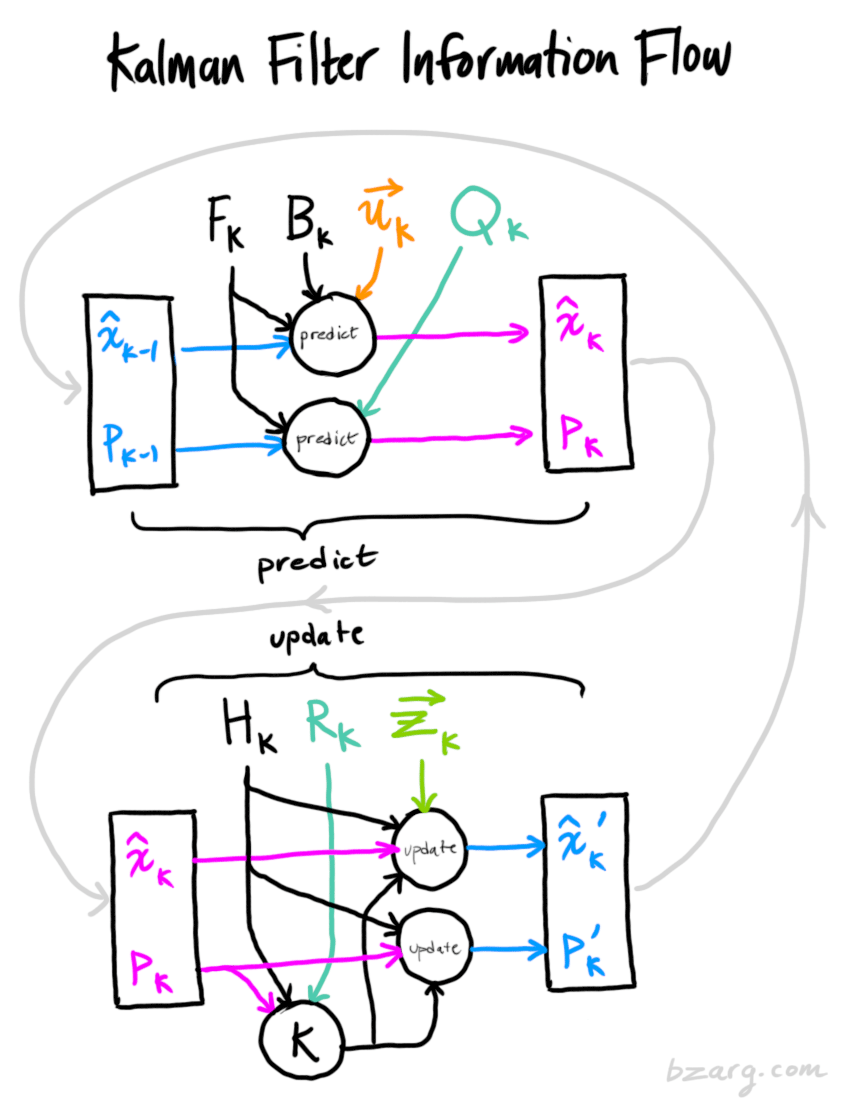
\includegraphics[scale=0.3]{images/kalflow}
\caption{Diagram showing the update in Kalman filter\\ credits: \url{http://www.bzarg.com/p/how-a-kalman-filter-works-in-pictures/}}
\end{figure}

The prediction step is given by the equation
\begin{equation}
\hat{x_k} = \mathbf{F_k} \hat{x}_{k-1} + \mathbf{B_k} \vec{u_k}
\label{eqn:stateestimate}
\end{equation}
\begin{equation}
\mathbf{P_k} = \mathbf{F_k} \mathbf{P_{k-1}} \mathbf{F_k}^T + \mathbf{Q_k}
\label{eqn:estimatecovariance}
\end{equation}

Equation \ref{eqn:stateestimate} is called the state estimate (a priori) equation. And equation \ref{eqn:estimatecovariance} is called the estimate (a priori) covariance. The significance of each variable is as follows:
\begin{itemize}
\item $\mathbf{F_k}$ is the state transition model which is applied to the previous state $\hat{x}_{k−1}$
\item $\mathbf{B_k}$ is the control-input model which is applied to the control vector $\vec{u}_k$
\item $\mathbf{P_k}$ error covariance matrix (a measure of the estimated accuracy of the state estimate)
\item $\mathbf{Q_k}$ the covariance of the process noise
\end{itemize}

Moving on to the update step, once we get the readings from the actual scenario, we need to update the model to update our belief about the scene. The update equations are given as
\begin{equation}
\label{eqn:kalmangain}
\mathbf{K'} = \mathbf{P_k} \mathbf{H_k}^T \left( \mathbf{H_k} \mathbf{P_k} \mathbf{H_k}^T + \mathbf{R_k} \right)^{-1}
\end{equation}

\begin{equation}
\hat{x'}_k = \hat{x}_k + \mathbf{K'} \left( \vec{z}_k - \mathbf{H_k} \hat{x}_k \right)
\label{eqn:posterioristateestimate}
\end{equation}

\begin{equation}
\mathbf{P'_k} = \mathbf{P_k} - \mathbf{K'}  \mathbf{H_k} \mathbf{P_k}
\label{eqn:posterioriestimatecovariance}
\end{equation}

where,
$$ \vec{z}_k = \mathbf{H_k} \hat{x}_k + \vec{v}_k$$
$$ \vec{v}_k \approx \mathcal{N}(0, \mathbf{R_k})$$

The equation \ref{eqn:kalmangain} is called the Kalman gain of the filter. The equation \ref{eqn:posterioristateestimate} is the updated (a posteriori) state estimation of the filter. And the equation \ref{eqn:posterioriestimatecovariance} is known as the updated (a posteriori) state covariance equation. The variables used in these equations are described below:

\begin{itemize}
\item $\mathbf{H_k}$ is the observation model which maps the true state space into the observed space
\item $\vec{v}_k$ is the observation noise
\item $\mathbf{R_k}$ is the covariance of observation noise which is assumed to be zero mean Gaussian white noise
\end{itemize}

After applying Kalman filter, the face detection becomes continuous and smooth to be used for dynamic perspective.

\subsection{Finding viewing angle of user}
The viewing angle is one of the critical measurements for creating a dynamic perspective system. After applying the Kalman filter to smoothen the face detection, we need to find the viewing angle with respect to the camera. Since all the coordinates are in image frame of reference, the angle can be found by using the following equations. 
\begin{equation}
\theta_x = tan^{-1} \left( \frac{x_f - \frac{W}{2}}{f_x} \right)
\label{eqn:thetax}
\end{equation}
\begin{equation}
\theta_y = tan^{-1} \left( \frac{y_f - \frac{H}{2}}{f_y} \right)
\label{eqn:thetay}
\end{equation}

In equation \ref{eqn:thetax} and \ref{eqn:thetay}, $(x_f, y_f)$ is the location of the centroid of the user's face. Image size is $W \times H$. $f_x$ and $f_y$ are the focal length of the camera in pixels.

\begin{figure}
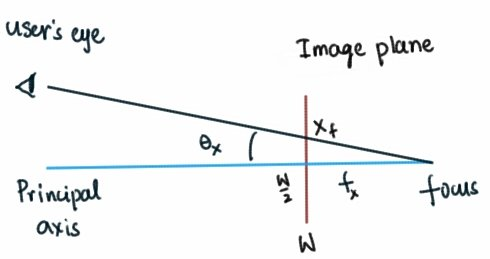
\includegraphics[scale=0.5]{images/view_angle}
\caption{The viewing angle of the user with respect to front camera on tablet}
\label{fig:viewangle}
\end{figure}

Figure \ref{fig:viewangle} shows the viewing angle of the user. The view angle is the angle subtended by the user's position with the principal axis of the camera. The focal length of the camera is found by using camera calibration in opencv \cite{calibration}.

\subsection{Inertial Measurement Unit}
    -Jenna
\subsection{Extended Kalman Filter}
    -Jenna
\section{Experiments}

\subsection{Camera calibration}
The camera calibration matrix is returned as
\begin{equation}
K = \begin{bmatrix}
f_x & \alpha_x & c_x\\
0 & f_y &  c_y\\
0 & 0 & 1
\end{bmatrix} = \begin{bmatrix}
145 & 0 & 930\\
 0 &145 & 601\\
0 & 0 & 1
\end{bmatrix}
\end{equation}

The value of the focal length is in terms of the pixels. The resolution of the camea is 1920x1280, and the principal axis seems to be almost at the center of the image.

\subsection{Kalman filter parameters}
The Kalman filter parameters are chosen as follows
$ \mathbf{F_k} = \begin{bmatrix}
1 & 0 & 1 & 0\\
0 & 1 & 0 & 1\\
0 & 0 & 1 & 0\\
0 & 0 & 0 & 1
\end{bmatrix} $,
$ \mathbf{H_k} = \begin{bmatrix}
1 & 0 & 0 & 0\\
0 & 1 & 0 & 0\\
\end{bmatrix} $

$$ \mathbf{Q_k} = \begin{bmatrix}
0.0001 & 0 & 0 & 0\\
0 & 0.0001 & 0 & 0\\
0 & 0 & 0.0001 & 0\\
0 & 0 & 0 & 0.0001
\end{bmatrix} $$

$$ \mathbf{R_k} = \begin{bmatrix}
0.1 & 0 \\
0 & 0.1\\
\end{bmatrix} $$

The initial estimates are given as

$ \hat{x}_{0} = \begin{bmatrix}
1\\1\\0\\0
\end{bmatrix} $,
$ \mathbf{P_{k0}} = \begin{bmatrix}
0.1 & 0 & 0 & 0\\
0 & 0.1 & 0 & 0\\
0 & 0 & 0.1 & 0\\
0 & 0 & 0 & 0.1
\end{bmatrix} $

$\mathbf{B_k}$ is not used, so its value is $\vec{0}$. For the update equation, the new detected point is used as position vector. In case of failure, $(\frac{W}{2}, \frac{H}{2})$ is used to update Kalman parameters.

\subsection{Face detection and Kalman Filter}
The positive parallax concept is demonstrated with a working demo on Samsung Galaxy Tab 10.1 (SM-P605L). the results are shown in figure \ref{fig:androiddemo} and \ref{fig:androiddemoanaglyph}. the system works real-time at 30fps. The equations used to generate the mask of size $(\frac{W}{2}, \frac{H}{2})$ is as follows

\begin{equation}
	X_{mask} = \frac{W}{4} - \frac{f}{2} \times \tan(\theta_x)
\end{equation}
\begin{equation}
	Y_{mask} = \frac{H}{4} + \frac{f}{2} \times \tan(\theta_y)
\end{equation}

Here $X_{mask}$ and $Y_{mask}$ are the top-left corner of the mask used for rendering the positive parallax. The mask has a constant size as we are not addressing the scale factor in this project.

Figure \ref{fig:androiddemoanaglyph} is an extension of the positive parallax concept which includes both the perspective change and the 3D rendering. The perspective change is because of the change in user's angle and the 3D rendering adds the depth perception to the perspective change making the system much more immersive. 


\begin{figure}
\begin{subfigure}{0.5\textwidth}
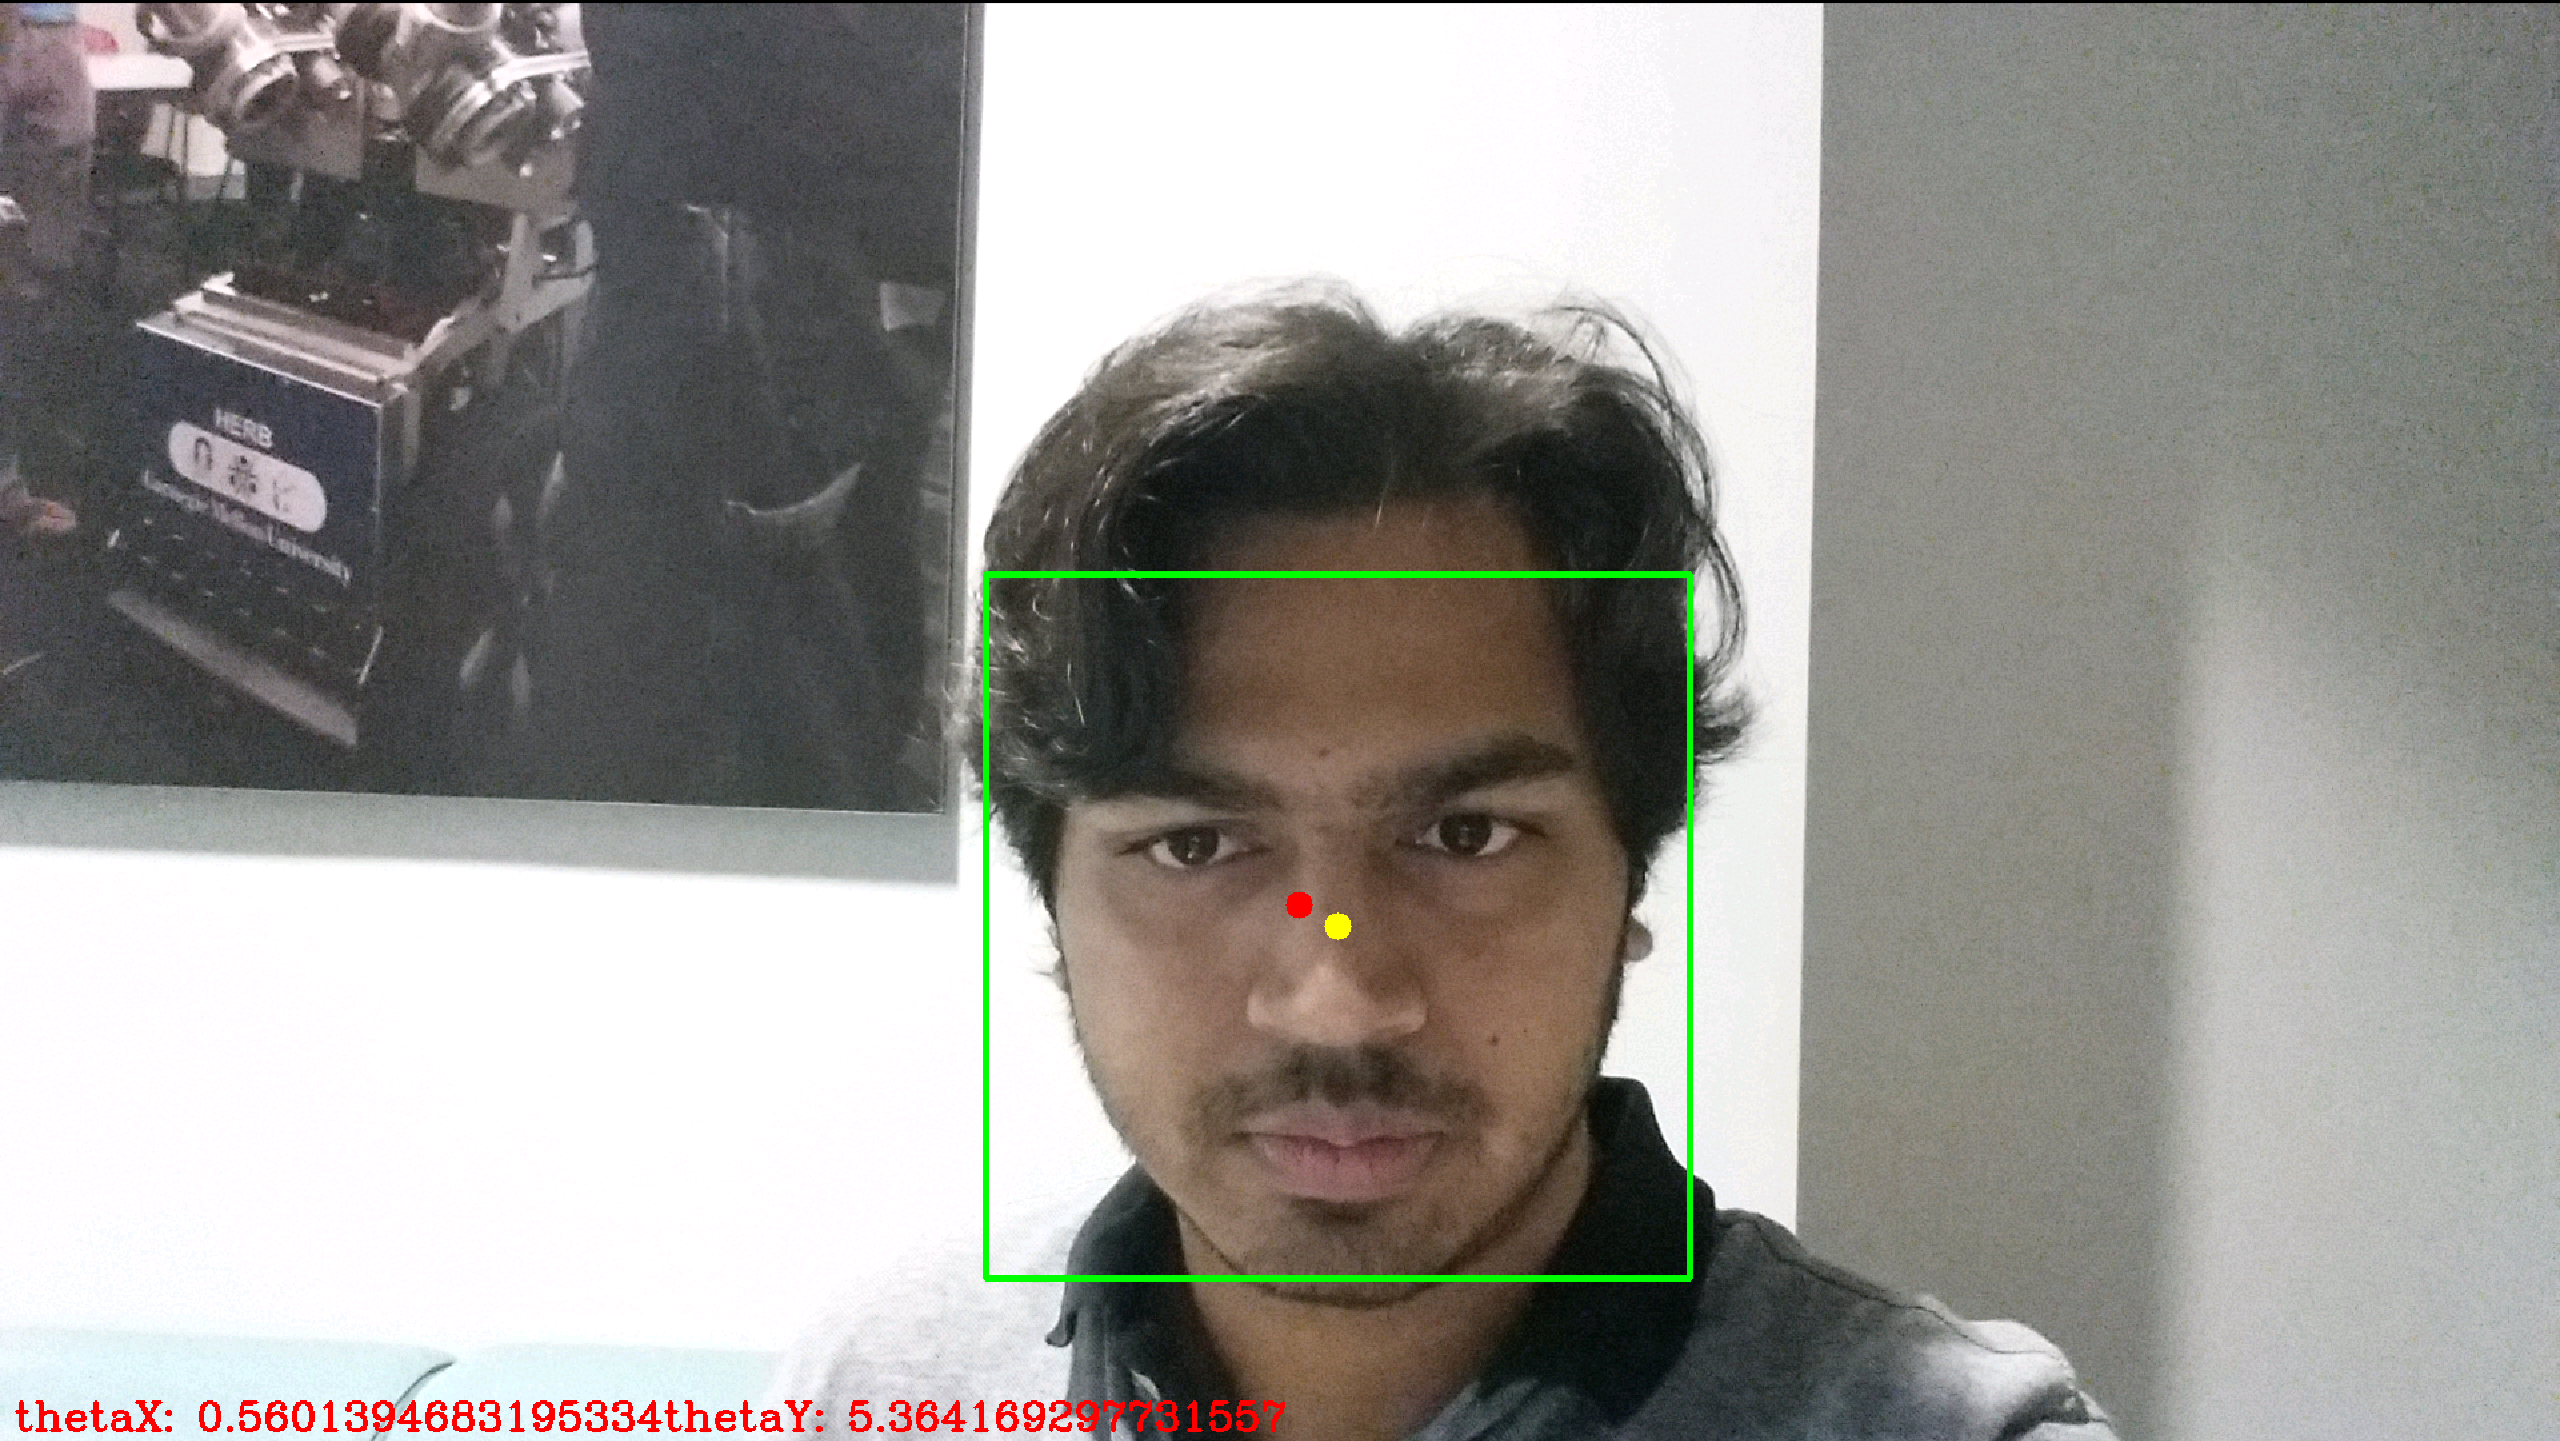
\includegraphics[scale=0.09]{images/jai}
\caption{Face tracking is done in 30fps with cascade classifier. $\theta_x$ and $\theta_y$ are displayed in degrees}
\end{subfigure}
\begin{subfigure}{0.5\textwidth}
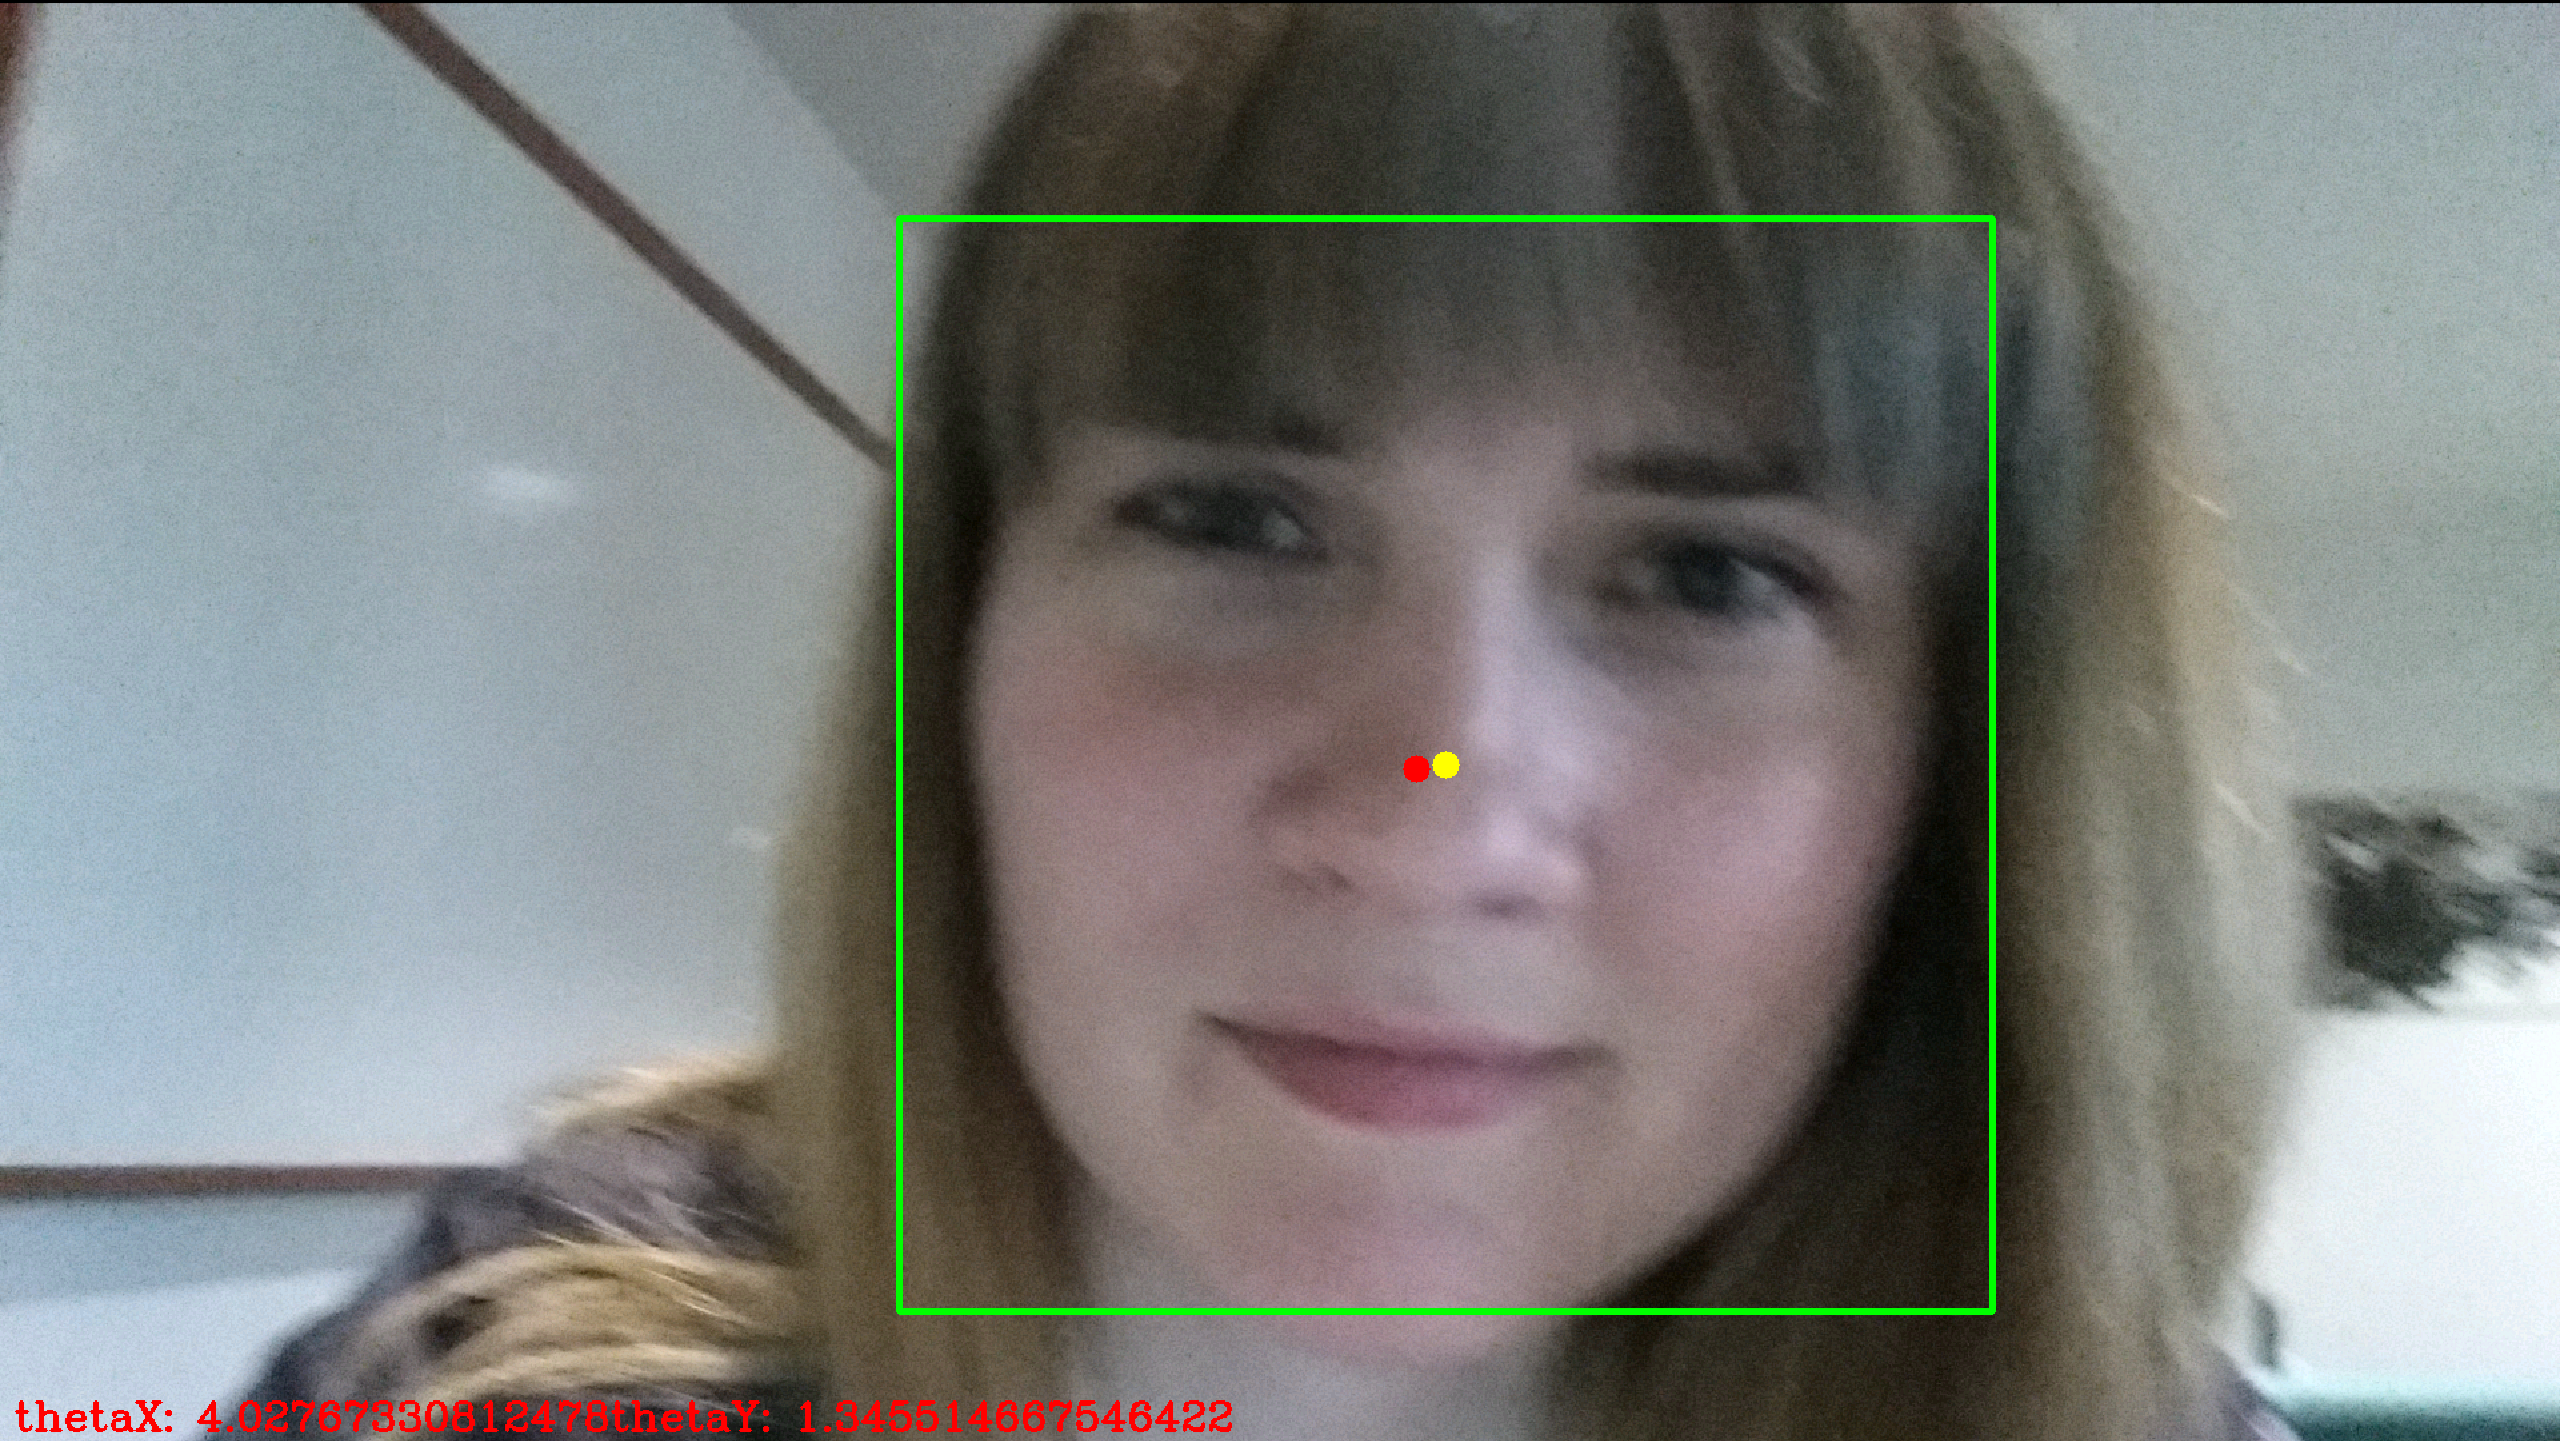
\includegraphics[scale=0.09]{images/jenna2}
\caption{Yellow dot shows the original centroid of face detection, red dot is the after Kalman filtering}
\end{subfigure}
\begin{subfigure}{0.5\textwidth}

\includegraphics[scale=0.09]{images/3dperspective_user_left}
\caption{UI change when the user views the tablet from left}
\end{subfigure}
\begin{subfigure}{0.5\textwidth}
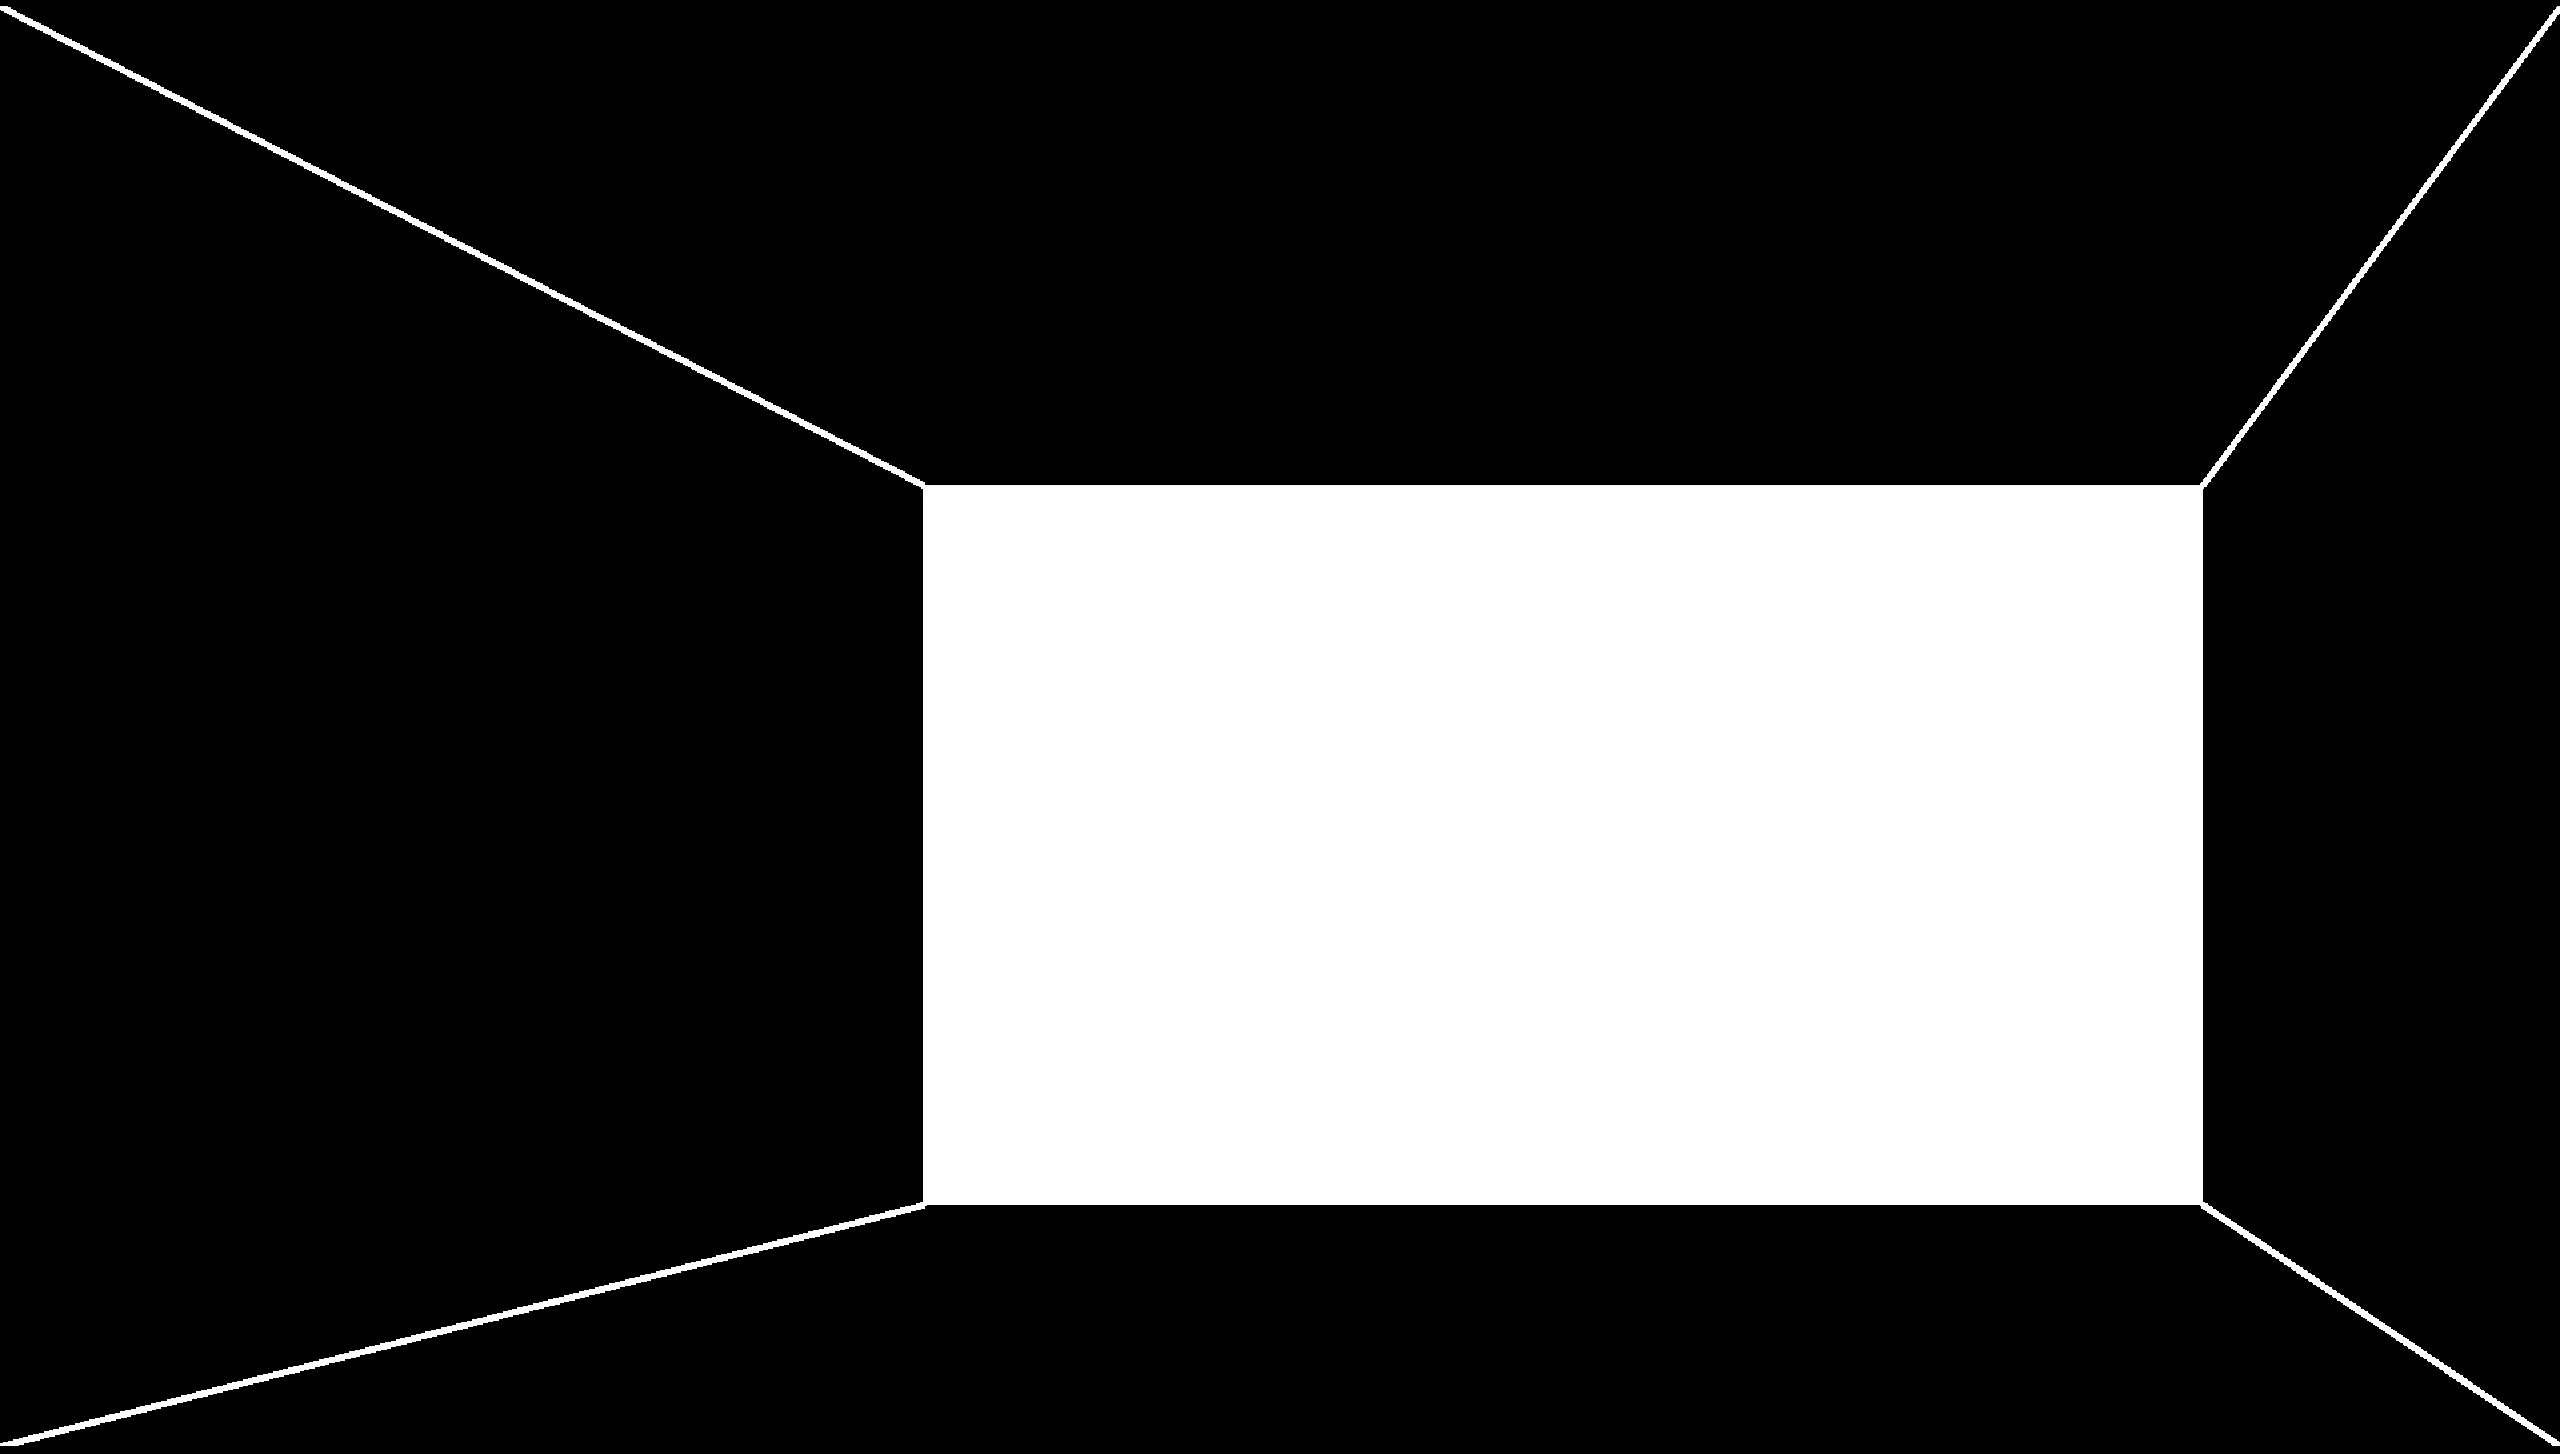
\includegraphics[scale=0.09]{images/3dperspective_user_right}
\caption{UI change when user views the tablet from right}
\end{subfigure}
\caption{Results of the working Andoid demo}
\label{fig:androiddemo}
\end{figure}

\begin{figure}
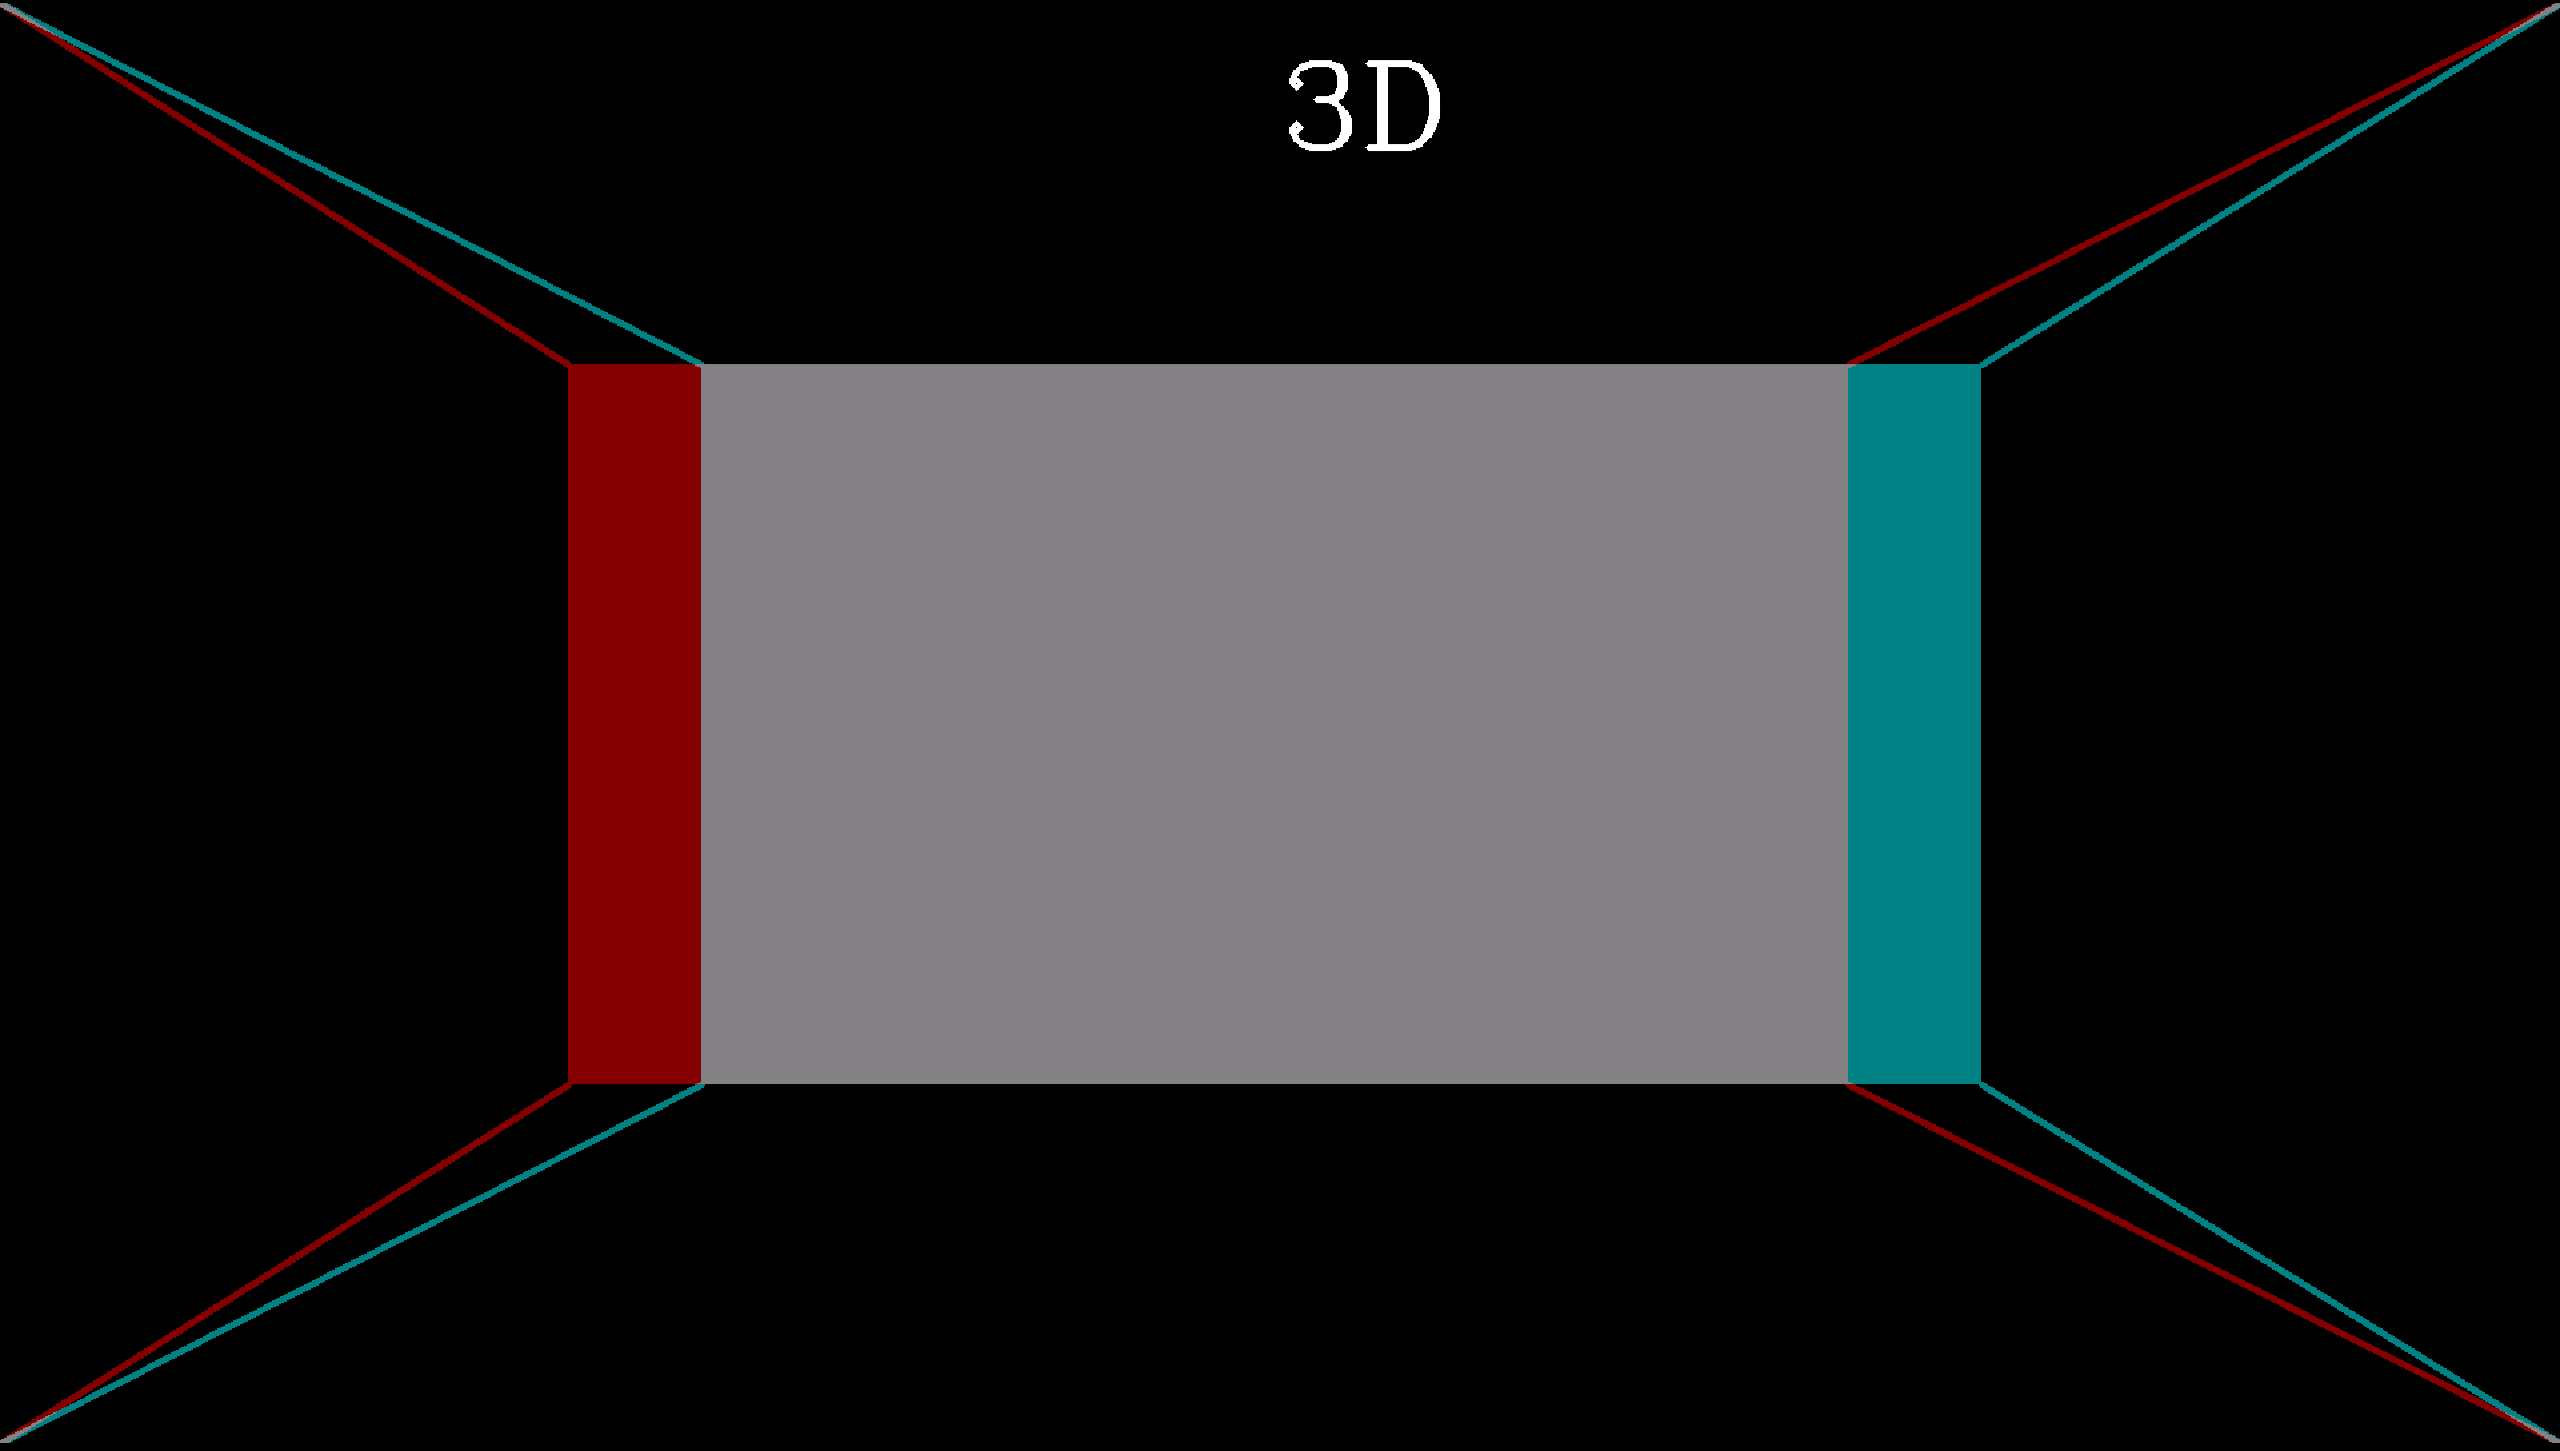
\includegraphics[scale=0.09]{images/anaglyph}
\caption{Result after adding the anaglyph demo to parallax}
\label{fig:androiddemoanaglyph}
\end{figure}

\subsection{IMU Experiments}
    -Jenna, make subsubsections as needed


\section{Conclusions}
    -Jai
{\small{
\begin{thebibliography}{11}

\bibitem{BusinessInsider}
Yarow, Jay. "Here's Why Apple Made That Motion-Effect For The Background Of The New IPhone Software." Business Insider. Business Insider, Inc, 25 Sept. 2013. Web. 11 Dec. 2015.

\bibitem{DigitalTrends}
Pelegrin, Williams. "Why Isn’t the Fire Phone Truly 3D? Amazon’s ‘Dynamic Perspective’ Tech Explained." \textit{Digital Trends}. Digital Trends, 18 June 2014. Web. 11 Dec. 2015.

\bibitem{jai}
J. Prakash and A. Vijayvargiya. A method for obtaining digital transparency in Electronic Devices, Indian Patent 4506/CHE/2014

\bibitem{calibration}
\url{http://docs.opencv.org/3.0-beta/doc/tutorials/calib3d/camera_calibration/camera_calibration.html}

\bibitem{kalman}
 Kalman, R. E. "A New Approach to Linear Filtering and Prediction Problems". \textit{Journal of Basic Engineering, 1960}

\end{thebibliography}

\end{document}

